% This is LLNCS.DEM the demonstration file of
% the LaTeX macro package from Springer-Verlag
% for Lecture Notes in Computer Science,
% version 2.4 for LaTeX2e as of 16. April 2010
%
\documentclass{llncs}
%
\usepackage{makeidx}  % allows for indexgeneration
\usepackage{amssymb}
\usepackage{amsmath}
\usepackage{algorithmic,eqparbox,array}
\usepackage{algorithm}
\usepackage{graphicx}
\usepackage{listings}
\usepackage{color}
\usepackage{multirow,booktabs,ctable,array}


    \definecolor{listcomment}{rgb}{0.0,0.5,0.0}
    \definecolor{listkeyword}{rgb}{0.0,0.0,0.5}
    \definecolor{listnumbers}{gray}{0.65}
    \definecolor{listlightgray}{gray}{0.955}
    \definecolor{listwhite}{gray}{1.0}


%\floatname{algorithm}{Procedure}
\renewcommand{\algorithmicrequire}{\textbf{Input:}}
\renewcommand{\algorithmicensure}{\textbf{Output:}}
\renewcommand{\algorithmiccomment}[1]{\hfill\eqparbox{COMMENT}{// #1}}
%
\begin{document}
%
\frontmatter          % for the preliminaries
%

\mainmatter              % start of the contributions
%
\title{ANTs and \'{A}rboles}
%\title{ANTs, \'{A}rboles, BRATS, and Brains}
%
\titlerunning{}  % abbreviated title (for running head)
%                                     also used for the TOC unless
%                                     \toctitle is used
%
\author{Nick Tustison\inst{1} \and Max Wintermark\inst{1} \and Chris Durst\inst{1} \and Brian Avants\inst{2}}

\authorrunning{N. J. Tustison, M. Wintermark, C. Durst, and B. B. Avants} % abbreviated author list (for running head)
\institute{University of Virginia, Charlottesville VA 22903, USA\\
\and
University of Pennsylvania,
Philadelphia PA  18104,USA
}

\maketitle              % typeset the title of the contribution

\begin{abstract}
Given the success of random forest approaches for segmentation, particularly for 
the BRATS 2012 tumor segmentation challenge, we implemented
a variant framework for our own research. 
The innovation of our methodology and implementation is characterized by 
the following four-fold contribution:
1) generation of
novel feature images in addition to what has been previously 
reported which significantly enhances classification,  2) 
concatenated application of random forest models for improved performance, 
3) the use of ANTsR (a packaging of the ANTs library plus 
additional analysis tools for
the R statistical project) for direct access to robust 
random forest functionality with parallelization, and 4) 
public availability of all scripts to recreate the 
leave-one-out evaluation study performed with the provided 
training data.
\keywords{ANTsR, Atropos, N4, R, random forests, segmentation}
\end{abstract}

\section{Introduction}

%Adoption of the random forest framework \cite{breiman1996} for learning computer vision tasks (e.g. \cite{viola2005}) has led to recent use within 
%the medical image analysis community for handling complex classification/regression tasks including normal brain segmentation \cite{yi2009},
%MS lesion segmentation \cite{geremia2011}, multimodal brain tumor segmentation
%\cite{zikic2012,geremia2012}, brain extraction \cite{iglesias2010}, 
%anatomy detection in computed tomography \cite{criminisi2013}, and
%segmentation of echocardiographic images \cite{verhoek2011}.
%A thorough introduction delving deeper into the more theoretical aspects 
%of random forests can be found in \cite{criminisi2011}.

The success of random forest (RF)-based approaches in the BRATS 2012 challenge, our 
own clinical research needs, and the lack of publicly available tools for such processing motivated the implementation that we describe herein.   Although we
borrowed many ideas from related previous work, our approach expands on this previous work in algorithmic and implementation terms both of which rely 
heavily on our Advanced Normalization Tools (ANTs)%
\footnote{
http://stnava.github.io/ANTs
} including its R packaging known as ANTsR.  
This includes concatenated application of RF models (one based on Gaussian mixture modeling (GMM), similar to previous efforts, used as input to the succeeding one based on maximum a priori estimation and Markov random fields (MAP-MRF)).  We then refine the resulting labeling using binary morphological processing.

%We first provide an overview of the workflow followed by a description of the different multi-modal feature images used to construct the random forest models.  We then detail the implementation including descriptions of the various scripts used to perform the evaluation study with the provided training data.  Finally, we provide the resulting label overlap metrics for the leave-one-out study performed for each training data cohort.

\section{Methods}

The proposed workflow for estimating tumor-based labeling from multi-modal images involves the following steps:
\begin{enumerate}
  \item Symmetric template construction \cite{avants2010}%
  \footnote{
  Implementation in the script {\tt antsMultivariateTemplateConstruction.sh}.
  }
 using the data described in \cite{landman2011}.
  \item Image preprocessing.
    \begin{itemize}
      \item Windowing image intensities (quantiles $[0.01,0.99]$).
      \item N4 bias correction \cite{tustison2010}.
      \item Rescaling intensity range to $[0,1]$.  
    \end{itemize}
  \item Stage 1 processing:
  \begin{itemize}
    \item generation of feature images,
    \item construction of the Stage 1 RF model and probability images.
  \end{itemize}
  \item Stage 2 processing:
  \begin{itemize}
    \item generation of single-modality MAP-MRF images using the Stage 1 RF probability images as spatial priors,
    \item construction of the Stage 2 RF model and labelings.
  \end{itemize}
  \item Refinement of Stage 2 labelings using binary morphological processing.
\end{enumerate}

%\subsection{Symmetric Template Construction}
%
%In order to better characterize deviations from normal
%multi-modal brain shape and appearance, several features were derived 
%using population-specific multivariate symmetric templates. 
%Further theoretical
%details can be found in \cite{avants2010}.

%Given $K$ image modality types for $N$ subjects,  
%${\mathbf I} = \{I_1,I_2,\ldots, I_K\}$, multivariate 
%template construction iterates between optimizing the set 
%of diffeomorphic transforms between the subjects and the 
%template, 
%$\left\{\left(\phi_1,\phi_1^{-1}\right),\ldots,\left(\phi_N,\phi_N^{-1}\right)\right\}$ 
%and constructing the 
%optimal multivariate template appearance 
%$\mathbf{J}=\{J_1,\ldots, J_K\}$ to minimize the
%cost function
%\begin{align}
%  \sum_{n=1}^N 
%        \left[ D \left( \psi(\mathbf{x}),\phi_1^n(\mathbf{x},1)\right)
%        + \sum_{k=1}^K \lambda_k \Pi_k \left(I_k^n\left(\phi_n(\mathbf{x},0.5)\right),J_k\left(\phi^{-1}_n(\mathbf{x},0.5)\right)\right)\right]
%\end{align}
%where $D$ is the shape distance,
%$D\left( \phi( \mathbf{x},0),\phi( \mathbf{x},1)\right) = \int_0^1 \| \nu(\mathbf{x},t)\|_L dt$
%dependent on the choice of linear operator, $L$, and $\nu$
%is the velocity field
%$\nu\left( \phi(\mathbf{x},t) \right) = \frac{d\phi(\mathbf{x},t)}{dt},\,\,\, \phi(\mathbf{x},0) = \mathbf{x}$.
%Each pairwise registration employing the similarity metric $\Pi_k$ can 
%be assigned a relative weighting, $\lambda_k$, to weight a particular
%modality's influence in the construction process.  

%We used the publicly available cohort associated with the multi-modal
%reproducibility study produced by Landman et al. \cite{landman2011}
%comprised of repeated acquisitions of several modalities for 21 normal 
%individuals.  Shown in Figure \ref{fig:symmetrictemplates} are slices
%from the resulting T1 symmetric template and derivative feature images.
%
%\begin{figure}
%  \centering
%  \begin{tabular}{ccccc}
%    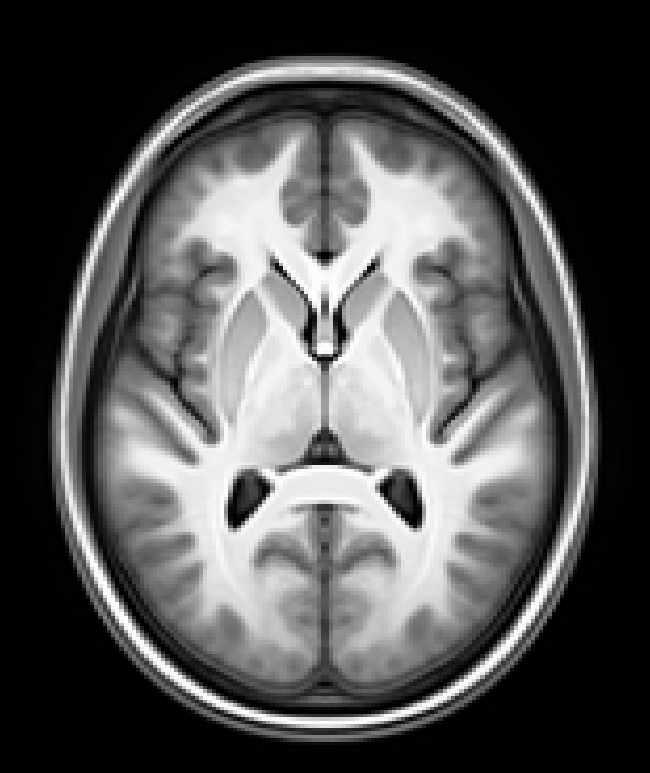
\includegraphics[height=40mm]{Figures/S_templateT1_140.png} &
%    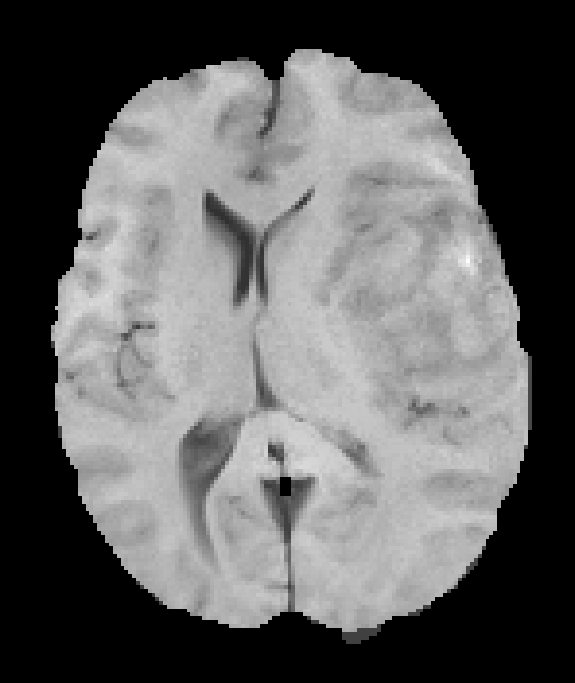
\includegraphics[height=40mm]{Figures/BRATS_HG0004_slice99.png} &
%    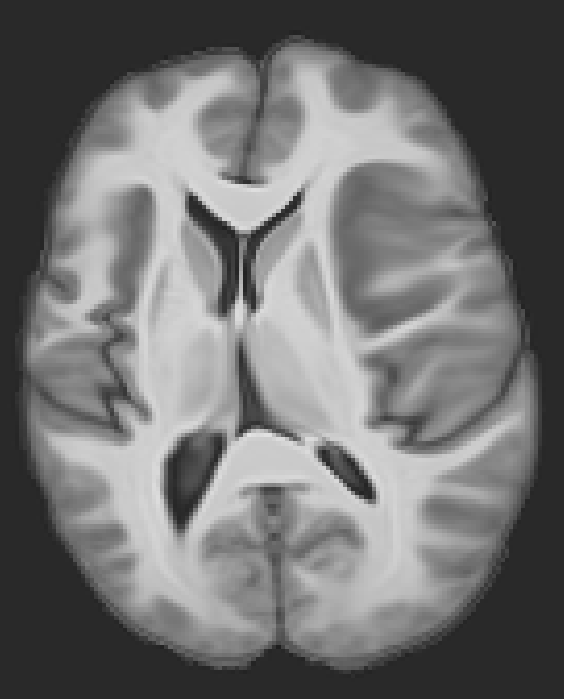
\includegraphics[height=40mm]{Figures/BRATS_HG0004_SymmetricTemplate3Warped_99.png} &
%    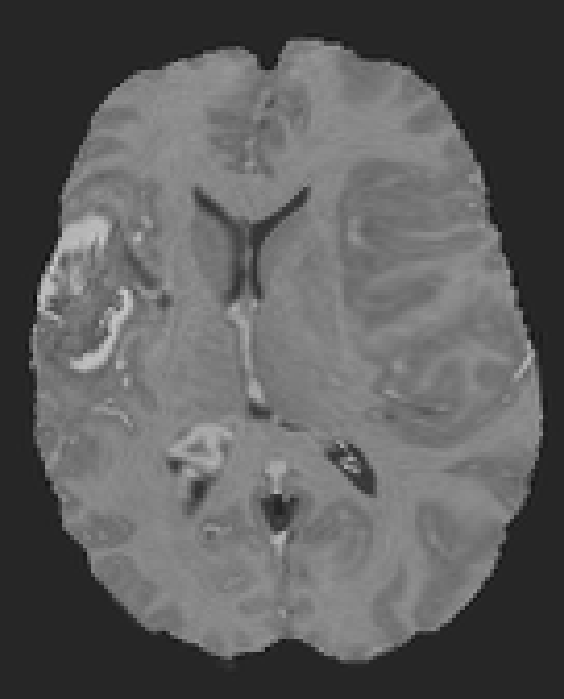
\includegraphics[height=40mm]{Figures/BRATS_HG0004_T1C_CONTRALATERAL_IMAGE_99.png} &
%    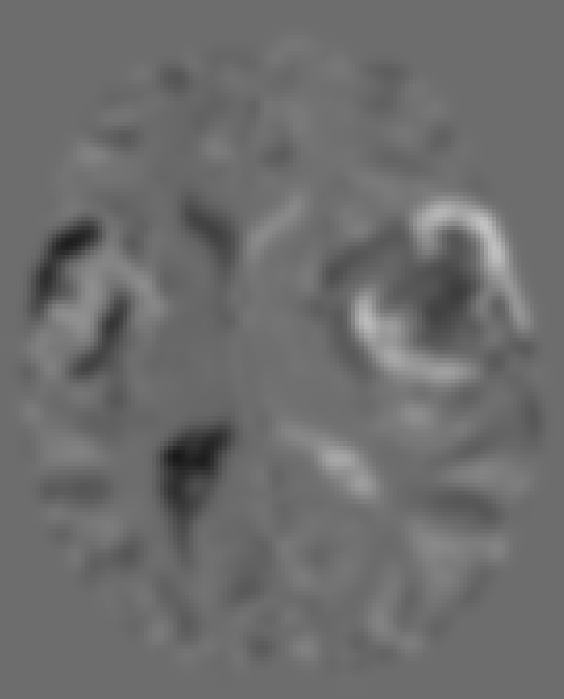
\includegraphics[height=40mm]{Figures/BRATS_HG0004_T1C_CONTRALATERAL_DIFFERENCE_99.png} \\
%        (a) & (b) & (c) & (d) & (e)
%  \end{tabular}
%  \caption{
%          }
%  \label{fig:symmetrictemplates}
%\end{figure}

%\subsection{Image Preprocessing}
%Although several studies have pointed out the importance of
%intensity normalization and bias correction, our experience 
%with the training data demonstrated a degradation in performance
%when one or both steps (using \cite{nyul2000} and N4 \cite{tustison2010},
%respectively) were performed.%
%\footnote{
%However, as we describe later, N4 is used in an interative scheme during the second
%stage in calculating the MAP-MRF segmentation for each subject.  
%} 
%For the first stage we windowed the image intensity
%for all images to be between the quantiles $[0.01,0.99]$
%and then performed N4 bias correction \cite{tustison2010}.
%This was followed by rescaling the resulting intensity range to $[0,1]$.  
%The set of feature images described in the next section are derived 
%from these ``corrected'' images.  

\subsection{Multi-Modal Feature Image Generation}

%Key to any supervised regression or classification protocol are the 
%selected features for training and subsequent testing.  

Based on previous
work and our own experience, we selected the following feature images
for our supervised segmentation framework:
\begin{itemize}
  \item Per modality (FLAIR, T1, T1C, T2)
    \begin{itemize}
      \item First-order neighborhood statistical images:
            mean, variance, skewness, and entropy. 
            Neighborhood radius $\in \{1,3\}$.
    \item GMM (stage 1) and MAP-MRF (stage 2) posteriors: CSF, gray matter, white 
          matter, necrosis, edema, non-enhancing tumor and enhancing tumor (or just 
          CSF, gray matter, white 
          matter, edema, and tumor for the simulated data).
    \item GMM (stage 1) and MAP-MRF (stage 2) connected component geometry 
          features:  distance to tumor core label, volume, volume to surface area ratio, eccentricity, and elongation
    \item Template-based:  symmetric template difference and 
          contralateral difference with Gaussian smoothing ($\sigma = 4$mm).
    \end{itemize}
  \item Miscellaneous: normalized Euclidean distance based on cerebral mask,
    log Jacobian image, and  (T1C - T1) difference image.
\end{itemize}

%\begin{figure}
%  \centerline{
%  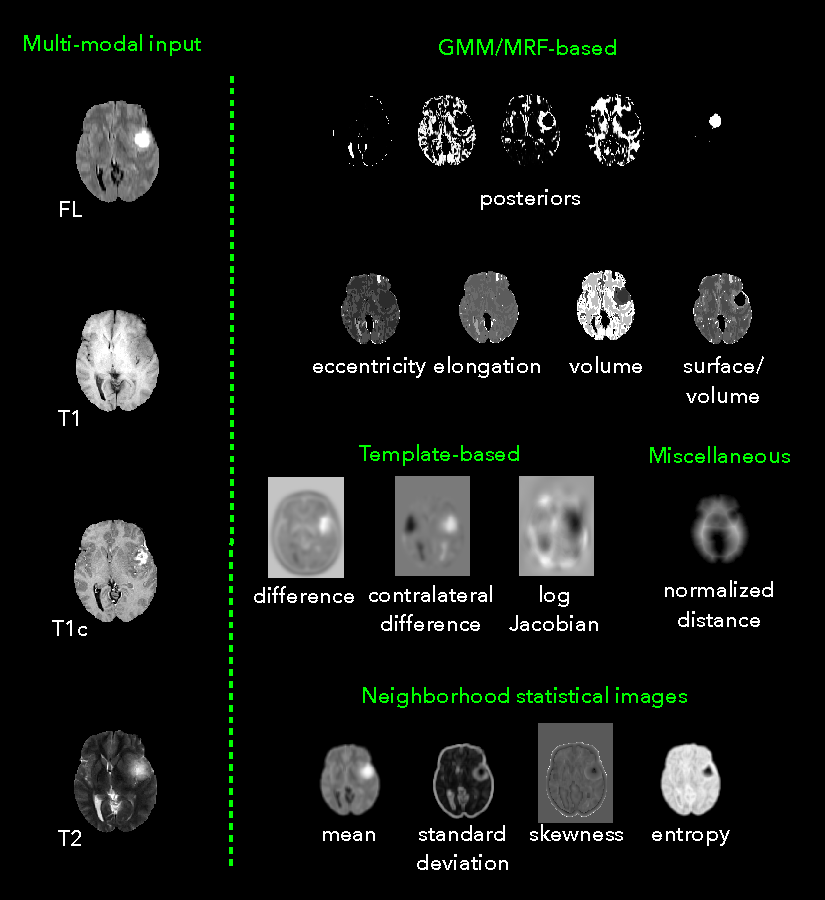
\includegraphics[width=125mm]{Figures/featuresImages2.pdf}
%  }
%  \caption{Sample feature images from the BRATS\_HG0004 data set.}
%  \label{fig:featureImages}
%\end{figure}

%For each modality, we create eight first-order statistical feature images,
%seven (or five for simulated data) posterior probability feature images, five geometry features generated from the GMM posterior probability images
%based on connected components, and two difference images using symmetric template
%construction.  Additionally, we create one normalized distance image 
%(the Euclidean distance image \cite{maurer2003} created from the skull-stripped 
%binary mask rescaled to the range $[0,1]$), a log Jacobian image based on normalization to the symmetric template, and a difference image between the T1 and T1 contrast image for a total of 4 modalities $\times (8 + 7 + 5 + 2) + 3$ feature images per modality $=$ 91 total
%feature images.  

Prior  cluster centers for specific tissue types learned from training data are used in the first stage to construct multiple GMM-based feature images \cite{avants2011}.  
%We do not use multivariate 
%Gaussians to specify tissue probabilities but rather incorporate each
%univariate probability map into the feature vector of the training
%data and let the random forest construction 
%process determine the optimal combination of such multivariate
%information.
The resulting spatial priors derived from application of the random
forest model for the first stage were used as input to an iterative
$n$-tissue N4 $\rightleftharpoons$ Atropos MAP-MRF segmentation protocol 
(encapsulated in the ANTs script 
\verb#antsAtroposN4.sh#) \cite{avants2011}.  These are used to 
create modified feature images for the second stage.

%One popular method for 
%determining the parameters of the GMM is maximum likelihood 
%estimation which can performed using the Atropos segmentation 
%tool \cite{avants2011}.  In contrast to previous generative
%modeling approaches for multi-modal tumor segmentation, we do not use multivariate 
%Gaussians to specify tissue probabilities but rather incorporate each
%univariate probability map into the feature vector of the training
%data.  As pointed out in \cite{menze2010}, multivariate modeling
%might obscure the distinct biological information provided by each 
%modality.  Instead, we let the random forest construction 
%process determine the optimal combination of such multivariate
%information.  

ANTs registration capabilities \cite{avants2011a} are also used to determine the transform from 
each subject to the symmetric template (using the tool \verb#antsRegistration#).  
This transform provides three 
sets of feature images:  the log Jacobian determinant image (assuming that the 
presence of tumor causes abnormal displacements), voxelwise intensity differences between each modality of each subject and the corresponding symmetric template component, and voxelwise contralateral differences.  
%The latter is calculated by warping each modality to the symmetric template, flipping the image contralaterally and warping it back to the subject space, and then calculating the difference image between the image and its contralateral counterpart.  
%This is very much influenced by earlier symmetric-based features described in \cite{geremia2011} although our approach accounts for a potentially deformed mid-sagittal plane caused by tumor growth.


%During the second stage, the probabilistic estimates
%of the white matter and gray matter labels were used to generate a
%``pure tissue weight mask'' to estimate the bias field 
%using N4 (although the resulting bias field estimation was used
%to correct the image within the entire cerebral mask).  Formally, this 
%involved generation of a probabilistic map defined as:
%\begin{align}
%  P_{pure\,\,tissue}(\mathbf{x}) = \sum_{i=1}^N P_i(\mathbf{x}) \prod_{j=1, j \neq i}^N \left( 1 - P_j(\mathbf{x}) \right)
%\end{align}
%where $N$ is the set of user-selected tissue labels (in our
%case $N=2$ consisting of the gray and white matter probability
%maps).
%Both rescaling and weighted bias correction were applied to produce
%the ``corrected images'' for the second stage resulting in
%modified features images for the second stage.  Note that we
%perform a similar iterative scenario for normal brain 
%segmentation \cite{avants2011} (encapsulated in the ANTs script 
%\verb#antsAtroposN4.sh#).

%Additionally, maximum posterior labeling from the GMM 
%processing  is used to determine the connected components for each label.  
%Geometric features (assigned voxel-wise) include the physical volumes 
%of each connected component including the volume to surface area ratio, 
%the elongation, and eccentricity. 
%Similarly, at the second stage, the probability maps determined from
%application of the stage 1 random forest model are used as spatial 
%priors for to construct MAP-MRF-based feature images analogous to the 
%stage 1 GMM feature images.  This is also performed using the Atropos
%segmentation tool available in ANTs.


\subsection{Implementation}

As mentioned previously, motivating this work were the limited public resources
for performing multi-modal tumor segmentation.  Github is used to make available all
scripts for the evaluation study as well as the source for this document%
\footnote{
https://github.com/ntustison/BRATS2013
}
in addition to ANTs,%
\footnote{
https://github.com/stnava/ANTs
}
ANTsR,%
\footnote{
https://github.com/stnava/ANTsR
}
and some additional utilities.%
\footnote{
https://github.com/ntustison/Utilities
}
The available scripts include:
\begin{itemize}
  \item \verb#createTruthLabels.pl# -- performs a 3-tissue segmentation of the tumor training data.  These three labels are then combined with the given labels. 
  \item \verb#createNormalizedImagesForCohort.pl# -- windows and rescales the images (commented out are previous attempts at N4 bias correction and intensity normalization).
  \item \verb#createFeatureImagesForCohort.pl# -- calculates the features images by calling \verb#createFeatureImages.sh# for each subject.
  \item \verb#runLeaveOneOutCrossValidation.pl#  -- calls \verb#createRandomForestModel.pl# for each subject using the training 
  data from the other subjects.
  \item \verb#createRandomForestModel.pl# -- calls the R script \verb#createModel.R#.
  \item \verb#applyTumorSegmentationModelForCohort.pl# -- creates the random
  forest probability maps for each label using \verb#applyTumorSegmentationModel.sh#.
  \item \verb#refineTumorSegmentationResultsForCohort.pl# -- refines the final labels from the random forest model using STAPLE.
  \item \verb#createFeatureImages.sh#  -- creates features images for a specific
  subject.
  \item \verb#applyTumorSegmentationModel.sh# -- given a random forest model (.RData), produces the subject-specific random forest probability images.
  \item \verb#createModel.R# -- R script interface to the \verb#randomForest# R package.  Provides optional parallelization with the \verb#snowfall# package.
  \item \verb#applyModel.R# -- R script interface to the \verb#randomForest# R package.  Provides optional parallelization with the \verb#snowfall# package.
  \item \verb#createCSVFileFromModel.R# -- produces a csv file containing a data frame of feature images.
  \item \verb#plotVariableImportance.R# -- plots feature importance given a random forest model.
\end{itemize}
%Although the perl scripts are specific to running jobs on the cluster at the 
%University of Virginia, they can be easily adapted to run on one's own platform.


%The ANTsR package (which also contains ANTs) is publicly available on the github project hosting service.%
%\footnote{
%https://github.com/stnava/ANTsR
%}
%Prior to installation of ANTsR, several external R packages
%need to be installed including: \verb#Rcpp#, \verb#signal#, \verb#timeSeries#, 
%\verb#mFilter#, \verb#doParallel#, \verb#robust#, \verb#magic#, \verb#knitr#, \verb#pixmap#, 
%\verb#rgl#, \verb#misc3d# which is facilitated by the 
%\verb#install.packages()# mechanism.  Additionally, in order
%to perform the supervised brain segmentation as described 
%in this work, one would need to also install 
%\verb#randomForest#, \verb#snowfall#, \verb#rlecuyer#, and \verb#ggplot2#. 
%The multivariate template construction is done using \verb#antsMultivariateTemplateConstruction.sh#, available in the ANTs \verb#Scripts# directory which permits parallel processing on
%an individual workstation or on a large computational cluster.

%\newpage
%
%%*** Authors: send us names and affiliations of your co-authors (ie. the co-authors from your abstract) using the following latex format:
%\author[label1,label2]{<author name>} %% use the full name, without abbreviating the first name  
%\address[label1]{<address>}  
%\address[label2]{<address>}

\author[label1]{Nicholas J. Tustison}
\author[label1]{Max Wintermark}
\author[label1]{Christopher R. Durst}
\author[label2]{Brian B. Avants}
\address[label1]{Department of Radiology and Medical Imaging, University of Virginia, Charlottesville, VA}
\address[label2]{Penn Image Computing and Science Lab, Department of Radiology, University of Pennsylvania, Philadelphia PA}

Given the success of random forest (RF)-based approaches in the BRATS 2012 
challenge, we employed RFs to produce a completely automated,
multi-modality brain segmentation framework.  However, differences from 
related work include an expanded feature image set, concatenated RF
modeling, and an open source implementation%
\footnote{
https://github.com/ntustison/BRATS2013
}
heavily dependent on the Advanced Normalization Tools (ANTs)%
\footnote{
http://stnava.github.io/ANTs
} repository including its R packaging (ANTsR).%
\footnote{
http://stnava.github.io/ANTsR
}
It is the latter open source aspect of our work which 
significantly motivated our participation in BRATS 2013 
as it provides a reproducible and publicly available framework 
for performing such an important task in neuroimaging 
\cite{ince2012}.

%*** Algorithm and data:  describe image features, classifiers, and spatial regularization (if these categories are meaningful for your approach). Name key parameters of your algorithm and their influence and mention if your algorithm needs manual input. Please also mention any additional preprocessing (normalization? registration?) and how you dealt with multichannel information and multiclass problem in case there was anything special about it (describe the processing pipeline where you fuse information from different channels, for example). Please give us a rough idea about the computing time and tell us what part of the algorithm is consuming most it.

The workflow for estimating tumor-based labeling from multi-modal 
images involves the following steps:
\begin{enumerate}
  \item Symmetric multivariate template construction \cite{avants2010}
 using the data described in \cite{landman2011}.
  \item Image preprocessing:
    \begin{itemize}
      \item Windowing intensities (quantiles $[0.01,0.99]$).
      \item N4 bias correction \cite{tustison2010}.
      \item Rescaling intensity range to $[0,1]$.  
    \end{itemize}
  \item Stage 1 (GMM) processing:
  \begin{itemize}
    \item generation of feature images,
    \item construction of the Stage 1 RF model and probability images.
  \end{itemize}
  \item Stage 2 processing:
  \begin{itemize}
    \item generation of single-modality MAP-MRF images using the Stage 1 RF probability images as spatial priors,
    \item construction of the Stage 2 RF model and labelings.
  \end{itemize}
  \item Refinement of Stage 2 labelings using a heuristically-derived binary morphological processing protocol.
\end{enumerate}

We used the following feature images:
\begin{itemize}
  \item Per modality (FLAIR, T1, T1C, T2)
    \begin{itemize}
      \item First-order neighborhood statistical images:
            mean, variance, skewness, and entropy. 
            Neighborhood radius $\in \{1,3\}$.
    \item GMM (stage 1) and MAP-MRF (stage 2) posteriors: CSF, gray matter, white 
          matter, necrosis, edema, non-enhancing tumor and enhancing tumor (or a
          subset for the simulated data).
    \item GMM (stage 1) and MAP-MRF (stage 2) connected component geometry 
          features:  distance to tumor core label, volume, volume to surface area ratio, eccentricity, and elongation
    \item Template-based:  symmetric template difference and 
          contralateral difference with Gaussian smoothing ($\sigma = 4$mm).
    \end{itemize}
  \item Miscellaneous: normalized Euclidean distance based on cerebral mask,
    log Jacobian image, and  (T1C - T1) difference image.
\end{itemize}

Prior cluster centers for specific tissue types learned from training data are 
used in the first stage to construct multiple GMM-based feature images \cite{avants2011}.  
The resulting spatial priors derived from application of the RF
 model for the first stage were used as input to an iterative
$n$-tissue N4 $\rightleftharpoons$ Atropos MAP-MRF segmentation protocol 
These are used to create modified feature images for the second stage.
ANTs registration \cite{avants2011a} is also used to produce three sets of 
feature images:  the log Jacobian image, 
intensity differences between each modality of each subject 
and the corresponding symmetric template, and contralateral 
differences.  

All processing was performed
using the computational cluster at the University of Virginia.%
\footnote{
http://www.uvacse.virginia.edu
}
Timing measures (single-threaded) included $\sim$1.5 hours per subject for 
feature image creation with the bulk of time devoted to spatial normalization 
with the symmetric template.  Model
construction required $\sim$2 hours with prediction taking approximately
15 minutes per subject.

%*** Training and testing: describe how you trained your algorithm. Did you do a cross-validation for parameter adaption? Did you learn individual classifiers for each of the four sub-problems (high/low & real/sim). Did you use any other data sets for training or tuning? Finally, mention shortcomings of your algorithm that you became aware of (specific cases or general difficulties), and ideas about how to possibly overcome them. If you had specific reasons why you did not apply your algorithm to all test sets, please mention them as well.

Training was performed separately for both real and simulated data and 
high-grade versus low-grade tumor assessment resulting in four RF modeling/prediction
pathways. Training was limited to the 80 evaluation data sets 
provided by the organizers with evaluation employing a leave-one-out
strategy for each of the four groupings.



%
%\newpage



\section{Evaluation}

%\begin{figure}
%  \centerline{
%  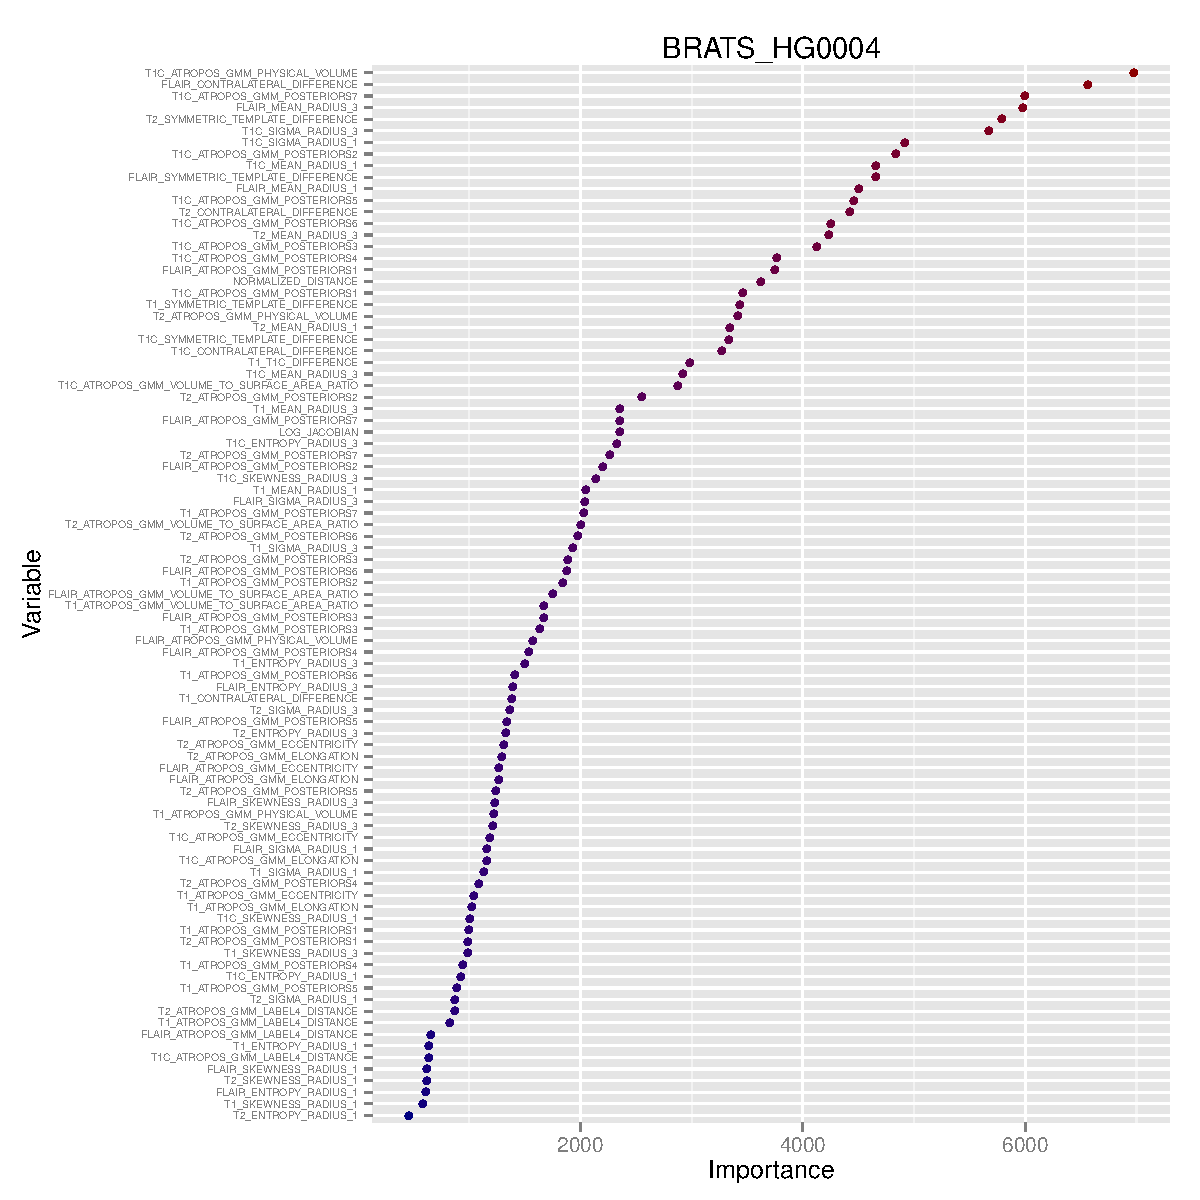
\includegraphics[width=150mm]{Figures/BRATS_HG0004GMM.pdf}
%  }
%  \caption{Relative variable importance plot of the different features used to construct the stage 1 random forest model for subject BRATS\_HG0004.}
%  \label{fig:importance}
%\end{figure}

A leave-one-out evaluation strategy was adopted for each of the four cohorts (high vs. low grade and real vs. simulated data).  
%The processing workflow described previously was applied to each subject whereby the remaining cohort members were used to train the random forest models which were then applied to that subject.  One of the benefits of random forests is that the training process can be used to produce a relative importance weighting of the individual features.  
The metrics for performance assessment were given by the organizers and include 
combining labels to assess overlap of complete tumor (labels 1--4), tumor core (labels 1,3, and 4), and enhancing tumor (label 4).  
The resulting assessment metrics are provided in Table \ref{table:brats}.  All processing was performed using the computational cluster at the University of Virginia.%
\footnote{
http://www.uvacse.virginia.edu
}
Given the number of subjects, all processing was single-threaded although multi-threading
can easily be employed.  The timing for the various stages were approximately as follows:
normalization (0.5 hours), Stage 1 feature image creation (8-10 hours due to image registration), Stage 2 feature image creation (1-1.5 hours), Stage 1 RF model construction (1-2 hours), and Stage 2 RF model construction (1-2 hours), and all remaining steps (0.5 hours).  
%For the on-site competition, the models will have already been built leaving the bulk of processing time devoted to creating the feature images.  I suspect that we can cut the current time in half using multi-threading and limiting the number of registration steps.

\begin{table*}
\caption{Scores from the MICCAI 2013 BRATs Evaluation Data}
\label{table:brats}
\centering
\begin{tabular*}{0.975\textwidth}{@{\extracolsep{\fill} } c c c c c c c c c c}
\toprule
{} & \multicolumn{3}{c}{Dice} & \multicolumn{3}{c}{Pos. predictive value} & \multicolumn{3}{c}{Sensitivity}\\
{} & complete & core & enhancing & complete & core & enhancing & complete & core & enhancing \\
\midrule
Real & {0.88} & {0.76} & {0.55} & {0.88} & {0.80} & {0.65} & {0.89} & {0.79} & {0.53} \\
Sim. & {0.89} & {0.90} & {0.00} & {0.82} & {0.88} & {0.00} & {0.99} & {0.93} & {0.00} \\
\bottomrule
\end{tabular*}
\end{table*}



\section{Discussion and Conclusions}

Our experience matches with previous research demonstrating good segmentation performance using random forests.  We found that a two-stage model construction incorporating a second MAP-MRF step while incorporating additional feature images to what has been proposed previously can significantly improve classification.  This includes symmetric template-based features, normalized Euclidean distance and log Jacobian images.  Additionally, we provide our implementation as open source.

\bibliographystyle{splncs03}
\bibliography{references}

\end{document}
